\documentclass[11pt]{article}
\usepackage[sc]{mathpazo} %Like Palatino with extensive math support
\usepackage{fullpage}
\usepackage{amsmath}
\RequirePackage[authoryear,sectionbib,sort]{natbib}
\bibliographystyle{amnatnat}
\linespread{1.7}
\usepackage{graphicx}
\usepackage[utf8]{inputenc}
\usepackage{lineno}
\usepackage{titlesec}
\titleformat{\section}[block]{\Large\bfseries\filcenter}{\thesection}{1em}{}
\titleformat{\subsection}[block]{\Large\itshape\filcenter}{\thesubsection}{1em}{}
\titleformat{\subsubsection}[block]{\large\itshape}{\thesubsubsection}{1em}{}
\titleformat{\paragraph}[runin]{\itshape}{\theparagraph}{1em}{}[. ]\renewcommand{\refname}{Literature Cited}

%%%%%%%%%%%%%%%%%%%%%
% Line numbering
%%%%%%%%%%%%%%%%%%%%%
%
% Please use line numbering with your initial submission and
% subsequent revisions. After acceptance, please turn line numbering
% off by adding percent signs to the lines %\usepackage{lineno} and
% to %\linenumbers{} and %\modulolinenumbers[3] below.
%
% To avoid line numbering being thrown off around math environments,
% the math environments have to be wrapped using
% \begin{linenomath*} and \end{linenomath*}
%
% (Thanks to Vlastimil Krivan for pointing this out to us!)

\title{Individual-to-population processes in the ecology and evolution of animal movement}

% This version of the LaTeX template was last updated on
% November 8, 2019.

%%%%%%%%%%%%%%%%%%%%%
% Authorship
%%%%%%%%%%%%%%%%%%%%%
% Please remove authorship information while your paper is under review,
% unless you wish to waive your anonymity under double-blind review. You
% will need to add this information back in to your final files after
% acceptance.

\author{Pratik R. Gupte$^{1,\ast}$ \\ 
        Christoph F. G. Netz$^{1,\ast}$ \\ 
        Franz J. Weissing$^{1}$}

\date{}

\begin{document}

\maketitle

\noindent{} 1. University of Groningen, Groningen 9747AG, The Netherlands.

\noindent{} $\ast$ Corresponding authors; e-mail: p.r.gupte@rug.nl OR pratikgupte16@gmail.com; c.f.g.netz@rug.nl

\bigskip

\textit{Manuscript elements}: EXAMPLE: Figure~1, figure~2, table~1, online appendices~A and B (including figure~A1 and figure~A2). Figure~2 is to print in color.

\bigskip

\textit{Keywords}: Examples, model, template, guidelines.

\bigskip

\textit{Manuscript type}: Article. %Or e-article, note, e-note, natural history miscellany, e-natural history miscellany, comment, reply, invited symposium, or historical perspective.

\bigskip

\noindent{\footnotesize Prepared using the suggested \LaTeX{} template for \textit{Am.\ Nat.}}

\linenumbers{}
\modulolinenumbers[1]

\newpage{}

\section{Abstract}

Predicting and managing population distributions is likely to be key to ensuring species survive the Anthropocene.
Classical individual-to-population models of distributions are rarely mechanistic, and do not account for rapidly changing landscapes, individual variation within animal populations, or the effects of ecological conditions on the evolution of movement rules.
Modern individual-based simulation models (IBMs) overcome these challenges by allowing multiple runs of the `tape of life' with both ecological and evolutionary mechanisms.
Here, we take a spatially explicit, IBM approach to model the evolution of individual movement rules in the context of optimal foraging on a landscape with discrete prey items.
We implement three plausible scenarios of how individuals are allowed to forage: (1) only forage, (2) only steal from other individuals, or only forage, and (3) condition foraging or stealing on environmental cues.
We examined the evolved movement rules and population distributions of each scenario in relation to landscape productivity, in order to distill insights for ecological modelling.
%%
First, we show that all three scenarios lead to activity distribution equilibria, and stealing, or kleptoparasitism evolves when permitted. 
% Differences in activity distributions among scenarios are more evident on high-productivity landscapes.
Second, individual movement rules evolve to distinguish between successful and unsuccessful foragers; this pre-adaptation is essential to the persistence of fixed and conditional kleptoparasitism.
Third, the functional response of intake to the presence of competitor individuals depends on competitor strategy.
Fourth, individuals caught on `clueless plateaus' without movement cues lead to populations not equalising intake rates across landscape quality gradients.
Finally, the effect of kleptoparasitism is to reduce prey extraction from the landscape and restore underlying spatial structure.
%%
Our study shows how IBMs can be used to gain insights into the ecological and evolutionary mechanisms behind individual-to-population distribution models.
Furthermore, the evolution of directed movement is a key prerequisite for the establishment of behaviours that allow animals to exploit discrete, unpredictable resources.
Mechanistic models of intermediate complexity should seriously be considered for predictive modelling populations which are expected to have many degrees of behavioural freedom.

\section{Introduction}

The proximate, ecological causes and consequences of animal movement are now understood in unprecedented detail, but the ultimate causes and large-scale consequences are poorly understood.
Animals, moving in response to internal and external stimuli, are key components of their ecosystems \citep{nathan2008,jeltsch2013}.
The consequences of myriad individual movement responses to local environmental cues result in large-scale emergent phenomena such as population distributions, community assembly, and landscape change \citep{jeltsch2013,schlagel2020}.
For instance, variation in dispersal movements between two species of bluebird \textit{Sialia sp.}, caused by differences in aggressiveness, results in unexpected cascading effects on inter-specific competition for habitat, and consequently on community composition \citep{duckworth2007}.
Similarly, there are strong feedbacks between the movement of consumers and their landscapes; while megafauna such as American bison \textit{Bison bison} engineer their ecosystems by facilitating plant growth and nutrient transfer \citep[][]{geremia2019,geremia2020,leroux2018}, predators can structure the same landscapes indirectly by affecting the movement of herbivores \citep[the landscape of fear;][]{leroux2018,kohl2018,brown1999}.
Yet movement behaviour leaves few clues as to its origins, and its long-term effects on populations and landscapes are yet more challenging to measure at an evolutionary scale.
This makes studying the ultimate evolutionary causes, and the long-term and large-scale consequences of animal movement, especially suitable for modelling studies.

Modelling the population-level outcomes of individual movement has long been studied within the framework of the archetypal individual-to-population model, \citeauthor{fretwell1970}'s (1970) ideal free distribution concept (IFD).
The IFD implicitly assumes an evolutionary rationale for optimal movement, that individuals wish to maximise their intake (here serving as a proxy for fitness) on a resource landscape.
Despite many extensions \citep[][]{tregenza1995,bernstein1988,cressman2006,meer1997}, and observed robustness \citep{sutherland1996} the IFD model is clearly unrealistic.
Two conceptual shortcomings --- no depletion by consumers and a static resource landscape, and the lack of an evolutionary component --- are especially grave.
Consumption by (mobile) animals can both facilitate \citep{geremia2019,leroux2018} and catastrophically alter resource landcapes [add grazers regime shift paper, elephant wp closure paper, geese grazing paper some bay in north america].
This is especially true when resources such as prey individuals are themselves mobile in response to consumption \citep{kohl2018}.
A population's evolutionary history on a landscape is also likely to shape individual responses to environmental cues at ecological timescales, as these are mostly drawn from a repertoire transmitted between generations.
For instance, ungulate populations occupying a habitat for generations track resource waves better than those recently translocated into a novel habitat, as resource tracking improves over evolutionary time \citep[][]{jesmer2018}.
These elements of biological realism rarely make for tractable analytical models, requiring a different approach.

An increasingly powerful individual-to-population approach is individual-based simulation modelling (IBM) \citep{deangelis2005,deangelis2018,grimm2017,railsback2020,huston1988}.
IBMs take a bottom-up view to encode many thousands of unique individuals with decision making mechanisms, and allow these individuals to move about and interact with their environment, and each other \citep{huston1988,deangelis2019}.
In this way, simple movement and behavioural rules can give rise to complex, population-scale emergent effects across spatial and conceptual scales, including localised population dynamics \citep{stillman2010}, small-scale group-foraging \citep{amano2006}, intermediate-scale disease-spread \citep{scherer2020,jeltsch1997}, and large-scale mass migration \citep{guttal2010}.
Conceptual and computational advances in IBMs \citep[][]{deangelis2018,deangelis2005} allow us to simulate a range of scenarios in unprecedented detail, and make general, testable predictions for population-level phenomena \citep[e.g.][]{spiegel2017}.
IBMs have mostly been employed to tackle the issue of spatial scale and complexity in animal movement \citep{spiegel2017}, they are equally well suited to modelling its evolution \citep{netz2020,guttal2010,getz2016,getz2015}.
It is important to include just enough realism and complexity in IBMs, so as to obtain interpretable outcomes for both populations and landscapes, at ecological and evolutionary scales.
For instance, \citeauthor{getz2015}'s (2015, 2016) work models unrealistic evolutionary processes, and \citeauthor{netz2020}'s multi-trophic model yields complex dynamics in which eco-evolutionary processes are difficult to disentangle.

Optimal foraging on a heterogeneous resource landscape is a scenario well suited to exploring individual-to-population processes in the ecology and evolution of animal movement.
The extensive literature on models in a foraging context, and their wide appeal provides a rich seam of inspiration \citep{vahl2005,vahl2005a,tregenza1995,sutherland1996,bernstein1988,cressman2006,garay2015}, and suggests broad applicability to real systems \citep{stillman2010,sutherland1996}.
Furthermore, an intermediate level of mechanistic complexity is easily included through several biologically plausible considerations: (1) discrete, depletable prey items with a handling time, (2) interference competition in the form of kleptoparasitism, and (3) interference as a fixed or conditional response.
Modelling discrete prey items which can be removed introduces exploitation competition, addressing an important shortcoming in analytical models \citep[][]{fretwell1970,cressman2006,garay2015}.
A handling time per item allows individuals to be susceptible to interference in the form of kleptoparasitism, which is a behavioural strategy common across animal taxa \citep[][]{iyengar2008}.
Encoding kleptoparasitism as a consistent, inherited behaviour, versus conditioning it on local environmental cues allows a comparison between plastic and implastic populations [a nice citation here?].
Recording the attributes of every individual over the population's history allows us to examine how movement responses evolve, and their effects on population behaviour at ecological timescales.
Finally, modelling a heterogeneous landscape allows the quantification of population distributions in relation to landscape quality, as well as landscape change (e.g. resource patchiness) [some citation here] in relation to the population's evolutionary trajectory.

Presenting the outcomes of such a model here, we show that --- 1. Consistent population-scale activity equilibria are often reached even in complex models of ecology and evolution, --- 2. The evolution of behaviour requiring individual interactions (e.g. kleptoparasitism) lags the evolution of movement towards individuals. This movement is itself only evolved when direct landscape quality cues are lacking, --- 3. The functional response of intake in relation to competitor individuals depends on the behavioural strategies of competitors, and not only on their number, --- 4. The aggregative response of individuals in relation to landscape quality is strongly determined by their behavioural strategy, --- 5. The evolution of kleptoparasitism, indirectly facilitated by resource-scarce landscapes, reduces resource harvesting and restores pre-existing spatial-structure in the prey landscape.

% The journal does not have numbered sections in the main portion of
% articles. Please refrain from using section references (à la
% section~\ref{section:CountingOwlEggs}), and refer to sections by name
% (e.g. section ``Counting Owl Eggs'').

\section{Methods: Simulation Model of Movement-Behaviour Co-Evolution}

Our model is an individual-based evolutionary simulation whose most basic components --- the environment size and shape, its gridded structure and each cell's capacity to hold multiple individuals, as well as the discrete conception of time within and between generations --- is taken from Netz et al. \textit{in prep.}.
We conceptualised the model and the scenarios around the behaviour of waders (\textit{Charadrii}, and especially oystercatchers \textit{Haematopus sp.}), which are extensively studied in an optimal foraging context \citep[e.g. ][]{vahl2005, vahl2005a, vahl2005b, ENS1990219}.
We simulated a fixed population with a fixed size of 10,000 individuals moving on a landscape of 512\textsuperscript{2} grid cells, with the landscape wrapped at the boundaries so that individuals passing beyond the bounds at one end re-appear on the diametrically opposite side.
Individuals have a lifetime of $T$ timesteps, with $T$ set to 400 by default.
After their lifetime, individuals reproduce and transmit their heritable traits proportional to their fitness over their lifetime.
The model code (in C++) can be found as part of the Supplementary Material in the Zenodo repository at \textbf{Zenodo/other repository here}.

\subsection{Three Foraging Strategiy Scenarios}

Our model considers three main scenarios of individual foraging strategies.
The \textbf{first scenario} is a forager-only case, in which individuals move about on the landscape and probabilistically find and consume discrete prey items.
Between finding and consuming a prey item, individuals must `handle' the prey for a fixed handling time $T_H$ which is constant across prey items.
Prey handling time $T_H$ is set at 5 timesteps by default.
The handling time dynamic is well known from many systems; for instance, it could be the time required for a wader to break through a mussel shell, with the handling action obvious to nearby individuals, and the prey not fully under the control of the finder.
We refer to such individuals as `handlers' for convenience.
Handlers are assumed to be fully absorbed in their processing of prey, and do not make any movements until they have fully handled and consumed their prey.
%%
The \textbf{second scenario} is a fixed-strategy case in which individuals inherit a fixed strategy, to either forage or to steal prey items from handlers, exclusively.
Agents that steal are termed kleptoparasites.
Kleptoparasites can steal from any handler, regardless of whether that handler acquired its prey by searching or theft.
Kleptoparasites are always successful in stealing from the handler they target; this may be thought of as the benefit of the element of surprise, a common observation in nature.
Having acquired prey, a kleptoparasite need only handle it for $T_H - t_h$ timesteps, where $t_h$ is the time that the prey has already been handled by its previous handler.
The targeted handler deprived of its prey is assumed to flee from the area, and does not make a further foraging decision.
Thus kleptoparasites clearly save time on handling compared to a forager, and the time saved increases with the handling time $T_H$ of the prey.
%%
The \textbf{third scenario} is a conditional-strategy case.
Individuals process local environmental cues and pick either the forager or kleptoparasite strategy to use in the next timestep.
Apart from the frequency of the choice, the actual foraging dynamics are the same as described in the fixed-strategy case.

\subsection{Movement and Foraging Decisions}

Individuals use cues available in timestep $t$ to predict their best move for the next timestep $t+1$, and the strategy associated with that move.
The movement decision is based on three local environmental cues: (1) the number of discrete prey items $G$, (2) the number of individuals handling  prey $H$ (referred to as `handlers'), and (3) the number of individuals not handling prey $P$ (referred to as `non-handlers').
Individuals are assumed to not be able to determine the intentions of others to either forage or steal, in scenarios 2 and 3.
The notation is chosen in keeping with Netz et al. \textit{in prep.}.
These cues are available to individuals in all three model scenarios.
%%
Individuals occupy a single grid cell on the environment at a time, and assign a suitability score $S$ incorporating $G$, $H$, and $P$ per cell to the nine cells in their Moore neighbourhood (including their current cell).
Following Netz et al. \textit{in prep.}, individuals calculate the cell-specific $S$ as
\begin{linenomath*}
    \begin{equation}
        S = m_gG + m_hH + m_pP
    \end{equation}
\end{linenomath*}
where the weighing factors for each cue $m_g$, $m_h$ and $m_p$ are genetically encoded and heritable between generations.
Individuals rank their Moore neighbourhood by $S$ in timestep $t$ and move to the highest ranked cell in timestep $t+1$.
%%
While individuals in scenario 1 only forage for prey items, individuals in scenario 2 use their inherited strategy to forage.
However, individuals in scenario 3 process the cell-specific environmental cues $G$, $H$, and $P$ to determine their next foraging strategy as
\begin{linenomath*}
    \begin{equation}
        strategy = 
    \begin{cases}
        {producer},& \text{if } f_gG + f_hH + f_pP + f_b \geq 0\\
        {scrounger},              & \text{otherwise}
    \end{cases}
    \end{equation}
\end{linenomath*}
where the cue weights $f_g$, $f_h$ and $f_p$, and the bias $f_b$ are also genetically encoded and heritable between generations.

Scenario 3 individuals make their foraging strategy choice for the next timestep after they have passed through the ecological dynamics of their current location.
This excludes individuals that have been stolen from are an important exception; these fleeing individuals are moved to a random cell within a Chebyshev distance of 5, and do not make a foraging decision there.
Thus kleptoparasitism not only gains individuals prey items while depriving the targeted individual, it also displaces a potential competitor.
All individuals move simultaneously, and attempt to implement the foraging strategy chosen for their new location (see below).

\subsection{Prey Environment and Ecological Dynamics}

Since our model was initially conceived to represent foraging waders, we developed a resource landscape based on mussels (family \textit{Mytilidae}) that are commonly found in inter-tidal systems.
Mussels beds share some important characteristics with other discrete prey items.
Firstly, mussels are immobile relative to their consumers, and their abundances are largely driven by extrinsic environmental gradients and very small-scale interactions \citep{dejager2020, dejager2011}.
Secondly, in common with many ecological systems \citep{levin1992}, mussels are not uniformly distributed across the inter-tidal mudflats, and are instead strongly spatially patterned into clusters (`beds') \citep{dejager2020, dejager2011}.
Thirdly, while prey or their signs in an area are often visible to consumers, consumers are not always certain of obtaining one of these prey.

We captured these essential aspects of prey dynamics when implementing the resource landscape on which our individuals move.
We modelled relative prey immobility and extrinsically driven abundance by assigning each grid cell of the resource landscape a constant probability of generating a new prey item per timestep, which we refer to as the cell growth rate $r$.
We modelled clustering in the abundance of prey by having the distribution of $r$ across the grid cells take the form of 1,024 uniformly distributed resource peaks with $r$ declining from the centre of each peak to its periphery (Figure X).
Effectively, the cell at the centre of each patch generates a prey item five times more frequently than the cells at the edges.
% Thus for a simulation-specific baseline $r_{max}$ = 0.03, the central cell of a resource peak  would have an $r_{centre} = 0.03$, and generate 3 items every 100 timesteps, compared with $r_{edge} = 0.006$, or 0.6 items generated in 100 timesteps.
We ran the simulation across a range of $r_{max}$ values (0.001 -- 0.25), which we considered a sufficiently broad range.
Cells in our landscape were modelled as having a carrying capacity $K$ of 5 prey items, and while a cell is at carrying capacity its $r$ is 0.
%%
We modelled near-perfect intermediate-range perception but uncertain short-range acquisition of prey by allowing individuals to perceive all prey items $G$ in a cell, but giving individuals which choose a forager strategy only a probability of finding one of these prey.
The probability of finding a prey item $p(success)$ is given as the probability of not finding any of $G$ prey each with a detection probability of $p_i$ = 0.2.
\begin{linenomath*}
    \begin{equation}
        p({success}) = 1 - \left(1 - p_i\right) ^ G
    \end{equation}
\end{linenomath*}

Since we model foraging events as occurring simultaneously, it is possible for more foragers to be considered successful in finding prey than there are discrete items in that cell.
We resolve this simple case of exploitation competition by assigning $G$ prey among some $N$ successful finders at random.
Foragers that are assigned a prey item in timestep $t$ begin handling it, and are considered to be handlers for the purposes of timestep $t+1$ (primarily movement and foraging decisions of other individuals).
% It is important to note that a forager that has converted into a handler in timestep $t$ is not an available target for kleptoparasites until timestep $t+1$.
Foragers that are not assigned a prey item are considered idle during timestep $t$, and are counted as non-handlers for $t+1$.

Kleptoparasites in the fixed- or conditional-strategy case face a slightly different challenge.
All kleptoparasites in a cell successfully steal from a handler, contingent on the number of handlers matching or exceeding the number of kleptoparasites in timestep $t$.
When the number of kleptoparasites exceeds handlers, handlers are assigned among kleptoparasites at random.
Successful kleptoparasites convert into handlers.
Unsuccessful kleptoparasites are considered idle, and are also counted as non-handlers for timestep $t+1$.
A handler that finishes processing its prey in timestep $t$ returns to the non-handler state and is assessed as such by other individuals when determining movements for $t+1$.

Individuals move and forage on the resource landscape for $T$ timesteps per generation, and $T$ is set at 400 by default. 
Handlers are immobile while they process prey for $T_H$ timesteps.

\subsection{Reproduction and the Evolution of Decision Making}

At the end of each generation, the population is replaced by its offspring, maintaining the fixed population size, and the decision-making weights which determine individual movement ($m_g$, $m_h$, $m_p$) and foraging strategy choice ($f_g$, $f_h$, $f_p$, $f_b$) are transmitted from parent individuals to offspring.
The total lifetime intake of individuals is used as a proxy of fitness, and the population's total fitness is its total intake.
%%
The number of offspring of each parent is proportional to the parent's share of the population fitness, and this is implemented as a weighted lottery that selects a parent for each offspring.
The decision-making weights are subject to independent random mutations with a probability of 0.001.
The size of the mutation (either positive or negative) is drawn from a Cauchy distribution with a scale of 0.01 centred on the current value of the weight to be mutated.
This allows for a small number of very large mutations while the majority of mutations are small.
%%
We recognised that spatial autocorrelation in the landscape coupled with limited natal dispersal can lead to spatial heterogeneity in evolved movement rules, as lineages adapt to local conditions \citep[][]{wolf2010}.
Furthermore, limited natal dispersal could lead to population-level movements due to differential reproduction that mirror shifts in resource abundance, rather than individual movement rules.
To ensure that global individual movement rules evolved, we intialised each offspring at a random location on the landscape, and also reset its total intake to zero.

\subsection{Simulation Output and Analysis}

\subsubsection{Ecological Equilibria}

We counted the number of times the forager or kleptoparasite strategy was used in each generation of our simulations, as well as the number of times no strategy could be used because individuals were handling a food item.
We refer to the ratio of time spent foraging, stealing, and handling as the population's activity budget.
We examined how the population activity budget developed over evolutionary time, and whether a stable ecological equilibrium was reached.
Furthermore, we counted the total population intake --- the number of items handled completely and consumed in each generation --- as a measure of population productivity.

\subsubsection{Evolution of Decision Making Weights}

To understand the evolutionary consequences of our simulation, we exported the the decision-making weights which determine individual movement and foraging strategy choice of each individual in every generation of the simulation.
We examined how the frequency of these weights changed over the simulation, i.e., how the weights evolved.
We visualised weights' evolution after scaling them between -1 and +1 using a hyperbolic tangent function, and binning the scaled values into intervals of 0.1.
We refer to these scaled and binned values as phenotypes for convenience.
Weights at or near -1 would represent the maximum evolved avoidance of an environmental cue (in relation to a movement weight) or the greatest evolved negative effect of a cue on choosing the foraging strategy (in relation to a strategy choice weight).
Similarly, weights at or near +1 represent the greatest evolved preference for or positive effect of a cue on the movement and strategy choice mechanism of an individual.

\subsubsection{Functional Response of Intake and Population Distribution}

In our simulation, individuals perceive and respond to the standing stock of prey items on a cell rather than its productivity, which they cannot sense directly.
This standing stock is unpredictable due to consumption by other individuals, and the movement (and consumption) of individuals is also unpredictable.
To understand the consequences of evolved movement rules, we must investigate how individual intake varies with the presence of items and other individuals.
Determining the functional response of intake to competitors, and the distribution of predators relative to prey \textit{sensu} \citet{meer1997} is a prevalent method in spatial ecology.
%%
Over the final ten generations of each simulation run, we summed the number of individuals and items on each cell, as well as the total intake on the cell.
We were able to record the number of individuals following a forager and kleptoparasite strategy, as well as intake due to foraging or stealing, separately.
This allowed us to determine the average per-capita, per-strategy intake on each cell, which we plotted against the number of competing individuals on the cell (Figure X).
Additionally, we plotted the average number of individuals following each strategy against the number of prey items on the cell (Figure Y).
In both cases, we used data only from the second half of each generation so as to capture the system in a state of ecological equilibrium.

While recognising that individuals move in response to their rapidly-changing prey landscape, it is useful to determine how individuals distribute along more slowly-changing productivity gradients; 
this is because these may often be easier to measure in the real world.
The ideal free distribution (IFD) and the matching rule robustly predict that individuals should distribute themselves such that intake rates are equalised over patches of similar productivity.
The large volume of pseduo-ecological data generated by our simulation allowed us to test whether intake rates were indeed equalised over the productivity gradient.
Having previously calculated the average numbers of each strategy, and the average per-captia intake for each strategy on each cell, we plotted both against the productivity of the cell (Figure Z).
Here too, we used data only from the second half of each generation to approximate ecological equilibrium.

\subsubsection{Landscape Effects of Kleptoparasitism}

optional: to be added

\paragraph*{Data Availability}

Simulation data used in this study are available on the Dryad/IRODS/Zenodo repository \textbf{REPOSITORY LINK HERE}; 
simulation code is available on Github and archived on Zenodo at \textbf{ZENODO LINK HERE}; 
data analysis and figure code is available on Github and archived on Zenodo at \textbf{ZENODO LINK HERE}.

\section{Results: Simulation Model Outcomes}

\subsection{Emergence of an Ecological Equilibrium}

All three simulation scenarios result in population level activity budget equilibria with stable proportions of foraging, kleptoparasitism, and handling (see Figure 2).
Populations reach this stable state within 100 generations, i.e., 10\% of evolutionary time (but see below).
Once a population reaches an activity budget equilibrium, it also reaches an intake equilibrium which is closely related to the proportion of handling (Figure 2).

In the foragers-only \textbf{scenario 1} case, the population is split among foraging and handling, while in the fixed-strategy \textbf{scenario 2}, kleptoparasitism rapidly increases to a stable proportion of the population's activity budget within 100 generations.
% This decrease is due to less kleptoparasitism, rather than more foraging; foraging forms between 10\% and 25\% of the population activity budget across $r_{max}$ in scenario 2.
However, at very high $r_{max}$ (0.25), kleptoparasitism is only approx. 10\% of the activity budget, and most individuals either forage or handle.
%%
In the conditional-strategy \textbf{scenario 3} populations largely handle prey, with kleptoparasitism and foraging relatively reduced (Figure 2).
In this scenario, activity budgets are unstable at low $r_{max}$, with strong oscillations in the proportion of foraging and kleptoparasitism.
Handling increases with $r_{max}$, and remains stable across generations (Supplementary Material Figure 1).
%%
Differences among scenarios in the proportion of handling translate to differences in total population intake.
While populations in all three scenarios have similar total intake at low $r_{max}$, forager-only populations have a higher intake than either fixed- or conditional-strategy populations, and conditional-strategy populations outperform fixed-strategy populations (Figure 3).

\subsection{Movement-Behaviour Co-Evolution}

\subsubsection{The Case of Exploitative Competition}

In scenario 1, movement and behavioural rules evolve to maximise intake in the presence of exploitation competition only, since individuals cannot steal.
Individuals evolve to move towards food items regardless of the simulation specific regrowth rate.
Individuals also evolve a movement preference for handling individuals at low and intermediate growth rates ($r_{max} < 0.1$); at high growth rates individuals evolve to be agnostic towards handlers.
Similarly, individuals are agnostic towards non-handling individuals at high growth rates, but evolve an avoidance at low -- intermediate growth rates.

\subsubsection{The Case of Kleptoparasitism}

\paragraph{Scenario 2}

In both scenarios 2 and 3, movement rules evolve to account for the additional pressure of interference competition in the form of kleptoparasitism.
In both scenarios and in common with scenario 1, individuals evolve to move towards food items across all $r_{max}$.
%%
In the fixed-strategy scenario 2, individuals evolve to move towards handlers at low to intermediate growth rates, but with an increasing proportion of individuals agnostic to handling individuals at higher growth rates.
Similarly, fixed-strategy individuals avoid non-handlers at lower growth rates, and are agnostic to non-handlers at higher growth rates.
%%
At lower growth rates, the majority of fixed-strategy individuals are kleptoparasites, and this proportion decreases in favour of the forager strategy with increasing $r_{max}$ until all individuals are foragers.

\paragraph{Scenario 3}

In the conditional-strategy scenario 3, individuals retain a preference for moving towards handlers across growth rates, unlike scenarios 1 and 2.
Conditional-strategy individuals also evolve a preference for moving towards non-handlers at high growth rates, while at low and intermediate growth rates they evolve to avoid non-handlers.
%%
The behavioural strategy of scenario 3 individuals is allowed to be conditional on local environmental cues, but unlike movement rules, few clear strategy choice rules evolve.
The only consistent signal is that of choosing a stealing strategy in the presence of handlers, with all scenario 3 individuals preferring to steal when possible, across $r_{max}$.

\subsection{Functional Response of Intake}

The foragers-only case presents a useful starting point: forager intake is invariant with individual (forager) density, and only declines at very high or low densities (Fig. 4.a,d).
Similarly, the functional response of both foragers and kleptoparasite strategies in the fixed-strategy and conditional-strategy case is hump-shaped, with an apparently `optimal' competitor density at which individual intake rates are maximised (Fig. 4.b,c).
Furthermore, the kleptoparasitic strategy's per-capita intake is always greater than that of the forager strategy (Fig. 4.b,c).
%%
However on separating potential competitors by strategy, we find that the individual intake of both strategies increases with increasing forager density (Fig. 4.e,f), but decreases with increasing kleptoparasite density (Fig. 4.g,h).
These consistently opposite responses to foragers and kleptoparasites explain why the overall functional response to all competitors appears hump-shaped.
%%
With growing forager densities, exploitative, scramble competition for prey items is increased, but foragers also accumulate on high-productivity cells, increasing average per-capita intake overall.
When kleptoparasites accumulate, however, interference competition results in both lower extraction (as only foragers extract prey) as well as lower intake, as the same item is repeatedly passed between individuals in stealing interactions.
Thus we show that taking the type of competition, and behavioural variation among individuals more generally into account is crucial to correctly understand the consequences of multiple competing individuals foraging on the same patch (or in the same group/in proximity to each other).

% \subsection{Aggregative Response and Population Distribution}

% Predicting the distribution of a population on a heterogeneous landscape is among the key goals of spatial ecology.
% While the ideal undertaking of such an endeavour involves fine-scale measurement of prey availability and predator densities, it is often much more realistic to find the aggregative response of individuals to a relatively static indicator of landscape quality.
% Our simulation data allowed us compare and contrast these approaches, and we examined the aggregative response of individuals in relation to both the number of discrete food items, as well as the underlying landscape productivity.

% \subsubsection{Aggregative Response of Predators to Prey}

% The aggregative response of predators to prey item density is strongly non-linear, and depends on the behavioural strategy as well as the regrowth rate.
% %%
% In scenario 1, at the reference $r_{max}$ of 0.1, predator density shows a humped response to predator density. 
% This arises from individual preference for cells with more prey items, and the consumption of prey by predators; prey are unlikely to accumulate on cells which are occupied by many predators.
% %%
% In scenario 2 at $r_{max}$ = 0.1, forager density is invariant with prey density except at very high prey densities, where predators are reduced.
% This latter is once again due to the feedback of predators on prey.
% However, kleptoparasite density increases nonlinearly with prey density, with many more kleptoparasites present at high prey densities than foragers.
% The ratio of kleptoparasites to foragers at high prey densities is signficantly higher at low $r_{max}$, in part due to the relatively greater prevalence of kleptoparasitism overall when landscape productivity is low.
% %%
% In scenario 3 for $r_{max}$ = 0.1, forager and kleptoparasite densities respond similarly to prey density, with a roughly 2:1 ratio of foragers to kleptoparasites.

\subsection{Population Distribution in Relation to Productivity}

We find that in the foragers-only case, individuals follow the matching rule in relation to grid-cell productivity, with more foragers on higher productivity cells (Fig. 5.a).
Individuals distribute such that their intake is equalised on cells with productivity above a threshold, while it is zero on cells below this threshold.
In this sense, the population appears to reach an ideal free distribution, as individuals can only increase their productivity by moving to cells above the threshold productivity, but not by moving any further up the productivity gradient.
In the fixed-strategy case, the aggregative response of foragers and kleptoparasites differs; forager counts peak on lower productivity cells and declines with further increases in productivity.
Kleptoparasite counts initially increase with cell productivity and then stabilise (Fig. 5.b).
In the conditional-strategy case, both foragers and kleptoparasite counts peak on intermediate productivity cells and then begin to decline (Fig. 5.c).
In the spatial context of our simulation, this translates to three distinct patterns with (1) individuals clustered on productivity peaks in scenario 1, (2) kleptoparasites dominating productivity peaks with fewer foragers in scenario 2, and (3) individuals using a forager strategy more frequently than a kleptoparasitic strategy on productivity peaks in scenario 3.
%%
We further find that there are appreciable differences between average and median counts of individuals of each strategy on cells, with the mean typically higher than the median.

\subsection{Landscape Effects of Kleptoparasitism}

Work in progress: -- add also landscape metrics etc

% If you have deposited data to Dryad, you should cite them somewhere in the main text (usually in the Methods or Results sections). A sentence like the following will do. All data are available in the Dryad Digital Repository (\citealt{CookEtAl2015}).

\section{Discussion}

\subsection{Relative Performance of Fixed and Conditional Strategies}

fixed strategies do nearly as well as conditional strategies at low growth rates --- conditional strategies pull ahead when resources are plentiful

\subsection{Evolution of Kleptoparasitism Requires Movement Pre-Adaptation}

The scrounging kleptoparasitic strategy evolves and is established in populations in some tens of generations, and emerges relatively quickly in the evolutionary history of populations (see Figure 2)
This rapid emergence and invasion is made possible by the pre-adaptation of individuals to use the kleptoparasitic strategy successfully.
\textbf{Scenarios 2} and \textbf{3} prior to the emergence and establishment of kleptoparasitism are identical to \textbf{scenario 1}, and all individuals are producers.
Producers evolve to move towards both items and handlers at most regrowth rates (Figure X), since these are cues to the immediate benefit, and the regrowth rate of a cell, respectively.
%%
For the kleptoparasitic strategy, the mapping of cues is reversed but the direction of preference remains the same.
To kleptoparasites, the number of handlers indicates the immediate resource abundance, while the number of items indicates the probability of resource generation, i.e., individuals converting into handlers.
This coincidental alignment of movement decisions with either behavioural strategy is essential to the persistence of kleptoparasitism.

The initial evolution of kleptoparasitism is then only conditional on the mutation of any one of the strategy weights to a sufficiently negative value such that the individual attempts to steal rather than search for prey.
At very high regrowth ($r_{max}$ = 0.25), the landscape is saturated with prey-items, and individuals can ignore the presence of handlers and evolve to move only in response to prey-items (`socially naive producers').
Under such circumstances in \textbf{scenario 2}, though strategy weight mutations lead to some few individuals using a fixed kleptoparasitic strategy, they do not move optimally for their strategy.
Thus kleptoparasitism as a fixed-strategy repeatedly evolves and goes extinct in high-productivity environments, as these individuals find themselves in a `desert of plenty'.
Under the same conditions in \textbf{scenario 3} however, a mixed foraging strategy allows individuals to be producers when appropriate, and yet steal a march on pure-producers when kleptoparasitism is possible.

\subsection{Functional Response Must Consider Competitor Behaviour}

functional response of intake ~ competition that does not consider individual strategies would lead to wrong conclusions --- facilitative effects may be entirely due to chance

\subsection{Clueless Plateaus Cause IFD Deviations}

individual consumption forms `clueless plateaus' --- individuals cannot find high productivity cells without cues --- this leads to undermatching

\subsection{Animal Behaviour Can Shape Landscapes}

Ssomething about klepts allowing landscape regrowth --- similar to predation --- landscape of fear etc etc


\section{Conclusion}


%%%%%%%%%%%%%%%%%%%%%
% Acknowledgments
%%%%%%%%%%%%%%%%%%%%%
% You may wish to remove the Acknowledgments section while your paper 
% is under review (unless you wish to waive your anonymity under
% double-blind review) if the Acknowledgments reveal your identity.
% If you remove this section, you will need to add it back in to your
% final files after acceptance.

\section{Acknowledgments}

The authors thank Hanno Hildenbrandt for contributing extensively to the coding of the simulation model \textit{Kleptomove};
Matteo Pederboni for contributing to the model's development; 
and members of the Modelling Adaptive Response Mechanisms Group, and of the Theoretical Biology department at the University of Groningen for helpful discussions on the manuscript.

\bibliography{kleptomove}

\newpage{}

\section{Appendix A: Supplementary Figures}

% In many cases, The American Naturalist allows authors to typeset 
% their own supplementary material in an author-supplied PDF. For author-
% supplied PDFs, please consult the AmNat_supp_template.tex document,
% available from https://www.journals.uchicago.edu/journals/an/instruct 
%
% By contrast, the Appendix instructions below apply to cases in which
% supplementary material is to be typeset by the AmNat editorial staff.
% That notably includes descriptions of methods, tables defining parameters,
% and other material necessary for reproducing the MS's results.
%
% Please reset counters for the appendix (thus normally figure A1, 
% figure A2, table A1, etc.).
%
% In certain cases, it may be appropriate to have a PRINT appendix in
% addition to (or instead of) an online appendix. In this case, please 
% name the print appendix Appendix A, and any subsequent appendixes (if 
% there are any) should be named Online Appendix B, Online Appendix C,
% etc.
%
% Counters for each appendix should match the letter of that appendix.
% For example, tables in Appendix C should be numbered table C1, table C2,
% etc. This applies to tables, equations, and figures.
%
% It's better not to use the \appendix command, because we have some
% formatting peculiarities that \appendix conflicts with.

\renewcommand{\theequation}{A\arabic{equation}}
% redefine the command that creates the equation number.
\renewcommand{\thetable}{A\arabic{table}}
\setcounter{equation}{0}  % reset counter 
\setcounter{figure}{0}
\setcounter{table}{0}

\subsection{Fox--dog encounters through the ages}

% The quick red fox jumps over the lazy brown dog. The quick red fox has always jumped over the lazy brown dog. The quick red fox began jumping over the lazy brown dog in the 19th century and has never ceased from so jumping, as we shall see in figure~\ref{Fig:Jumps}. But there can be surprises (figure~\ref{Fig:JumpsOk}).

% If the order and location of figures is not otherwise clear, feel free to include explanatory dummy text like this:

% [Figure A1 goes here.]

% [Figure A2 goes here.]

% \subsection{Further insights}

% Tables in the appendices can appear in the appendix text (see table~\ref{Table:Rivers} for an example), unlike appendix figure legends which should be grouped at the end of the document together with the other figure legends.

% \begin{table}[h]
% \caption{Various rivers, cities, and animals}
% \label{Table:Rivers}
% \centering
% \begin{tabular}{lll}\hline
% River        & City        & Animal            \\ \hline
% Chicago      & Chicago     & Raccoon           \\
% Des Plaines  & Joliet      & Coyote            \\
% Illinois     & Peoria      & Cardinal          \\
% Kankakee     & Bourbonnais & White-tailed deer \\
% Mississippi  & Galena      & Bald eagle        \\ \hline
% \end{tabular}
% \bigskip{}
% \\
% {\footnotesize Note: See table~\ref{Table:Founders} below for further table formatting hints.}
% \end{table}

% Lorem ipsum dolor sit amet, as we have seen in figures~\ref{Fig:Jumps} and \ref{Fig:JumpsOk}.

\newpage{}
\renewcommand{\theequation}{B\arabic{equation}}
% redefine the command that creates the equation number.
\renewcommand{\thetable}{B\arabic{table}}
\setcounter{equation}{0}  % reset counter 
\setcounter{table}{0}

\section{Appendix B: Additional Methods}

\subsection{Measuring the height of fox jumps without a meterstick}

% Pellentesque ac nibh placerat, luctus lectus non, elementum mauris. 
% Morbi odio velit, eleifend ut hendrerit vitae, consequat sit amet 
% nulla. Pellentesque porttitor vitae nisl quis tempus. Pellentesque 
% habitant morbi tristique senectus et netus et malesuada fames ac 
% turpis egestas. Praesent ut nisi odio. Vivamus vel lorem gravida 
% odio molestie volutpat condimentum et arcu (\citealt{tytler-mqos}). 

% \begin{equation}
% { \frac{1}{N_k-1} \sum \limits_{t=1}^{N_k} (M_{tjk} - \bar{M}_{jk})^2}
% \end{equation}

% \subsection{Quantifying the brownness of the dog}

% Pellentesque eu nulla odio (\citealt{Xiao2015,CookEtAl2015}). Nulla aliquam porta metus, quis malesuada orci faucibus quis. Suspendisse nunc magna, tristique sit amet sollicitudin nec, elementum et lacus. Sed vitae elementum mi. In hac habitasse platea dictumst. Etiam eu tortor elit. Sed ac tortor purus. Aliquam volutpat, odio sit amet posuere pretium, dolor ex interdum ante, sed luctus quam eros ac nulla. 

% \begin{equation}
% { (\sum \limits_{p=1}^P {n_{sp}})^{-1}\sum \limits_{p=1}^P {n_{sp}Q_{p}}}
% \end{equation}

\newpage{}

%%%%%%%%%%%%%%%%%%%%%
% Bibliography
%%%%%%%%%%%%%%%%%%%%%
% You can either type your references following the examples below, or
% compile your BiBTeX database and paste the contents of your .bbl file
% here. The amnatnat.bst style file should work for this---but please
% let us know if you run into any hitches with it!
%
% If you upload a .bib file with your submission, please upload the .bbl
% file as well; this will be required for typesetting.
%
% The list below includes sample journal articles, book chapters, and
% Dryad references.

\newpage{}

\section{Tables}
\renewcommand{\thetable}{\arabic{table}}
\setcounter{table}{0}

% \begin{table}[h]
% \caption{Founders of \textit{The~American Naturalist}}
% \label{Table:Founders}
% \centering
% \begin{tabular}{lll}\hline
% Early editor            & Years with the journal \\ \hline
% Alpheus S. Packard Jr.  & 1867--1886 \\
% Frederick W. Putnam     & 1867--1874 \\ 
% Edward S. Morse         & 1867--1871 \\ 
% Alpheus Hyatt           & 1867--1871 \\
% Edward Drinker Cope$^a$ & 1878--1897 \\
% J.~S. Kingsley          & 1887--1896 \\ \hline 
% \end{tabular}
% \bigskip{}
% \\
% {\footnotesize Note: Table titles should be short. Further details should go in a `notes' area after the tabular environment, like this. $^a$ Published the first description of \textit{Dimetrodon}.}
% \end{table}

\newpage{}

\section{Figure legends}

\begin{figure}[h!]
    \centering
    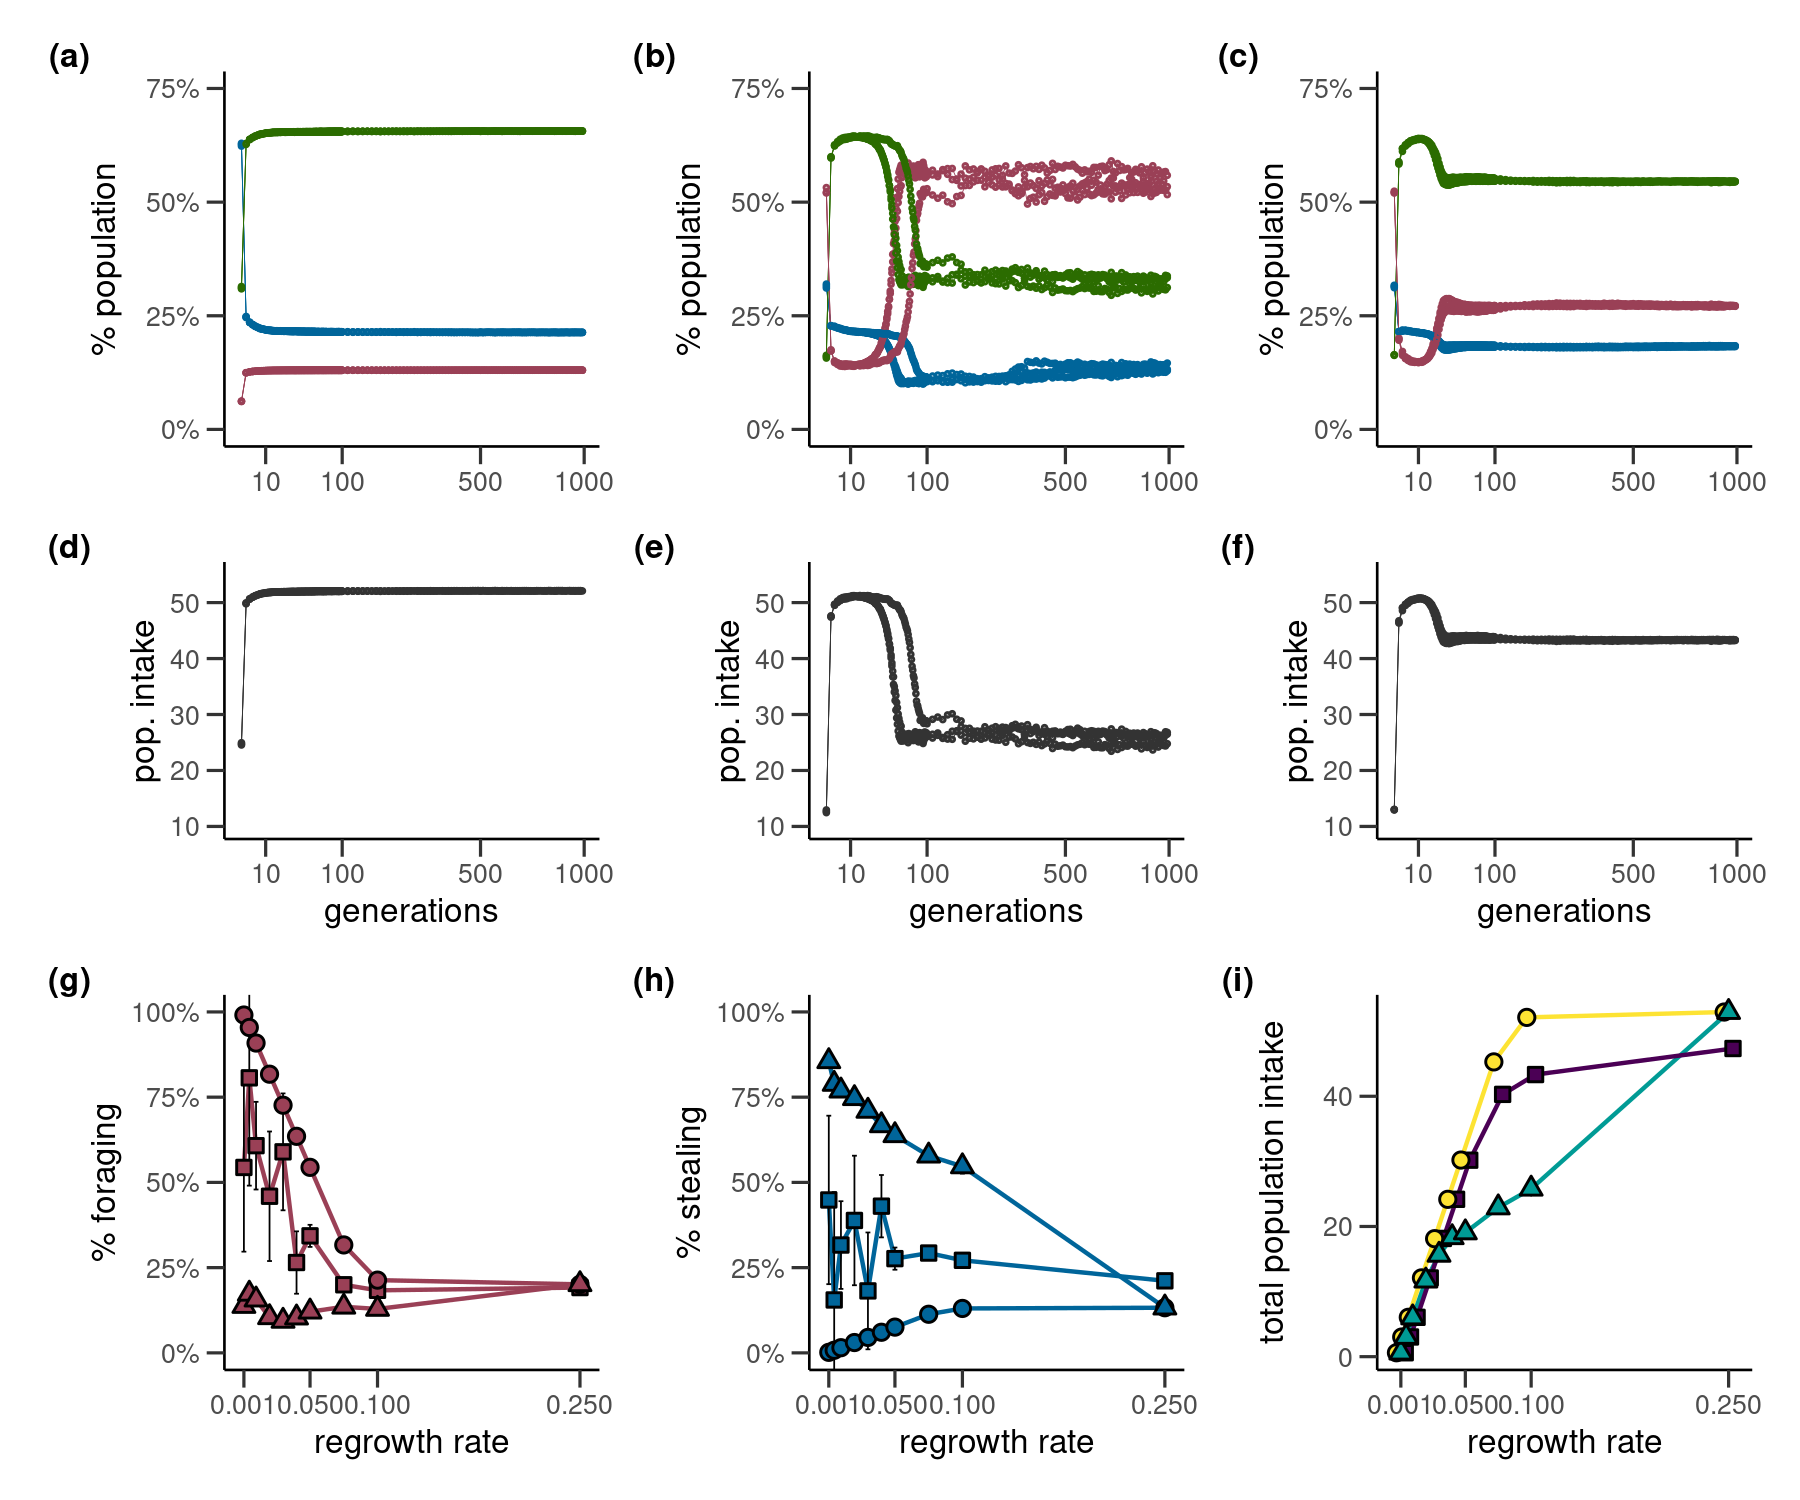
\includegraphics[width=0.90\textwidth]{figures/fig_02_equilibrium.png}
    \caption{Populations reach a stable state in their activity budgets early in their evolutionary history (blue = foraging, green = handling, red = stealing), and 
    activity equilibrium is associated with the intake (and thus fitness) equilibrium (black). Scenarios are shown at $r_{max} = 0.1$ and with a square-root transformed X-axis to show earlier generations more clearly; \textbf{(a, d)} forager-only, \textbf{(b, e)} fixed-strategy, and \textbf{(c, f)} conditional-strategy.
    \textbf{(g)} The proportion of foraging decreases a higher $r_{max}$, as more individuals are handlers.
    \textbf{(h)} Stealing decreases as a fixed strategy with increasing resources.
    \textbf{(i)} Total intake increases with increasing $r_{max}$. Fixed strategy populations outperform conditional strategies at the highest $r_{max}$ by switching to fixed foraging alone.
    Across (g, h, i) strategies are represented by symbols (circles = forager-only, triangles = fixed-strategy, squares = conditional-strategy). 
    }
    \label{Fig:EcologicalEquilibrium}
\end{figure}

\begin{figure}[h!]
    \centering
    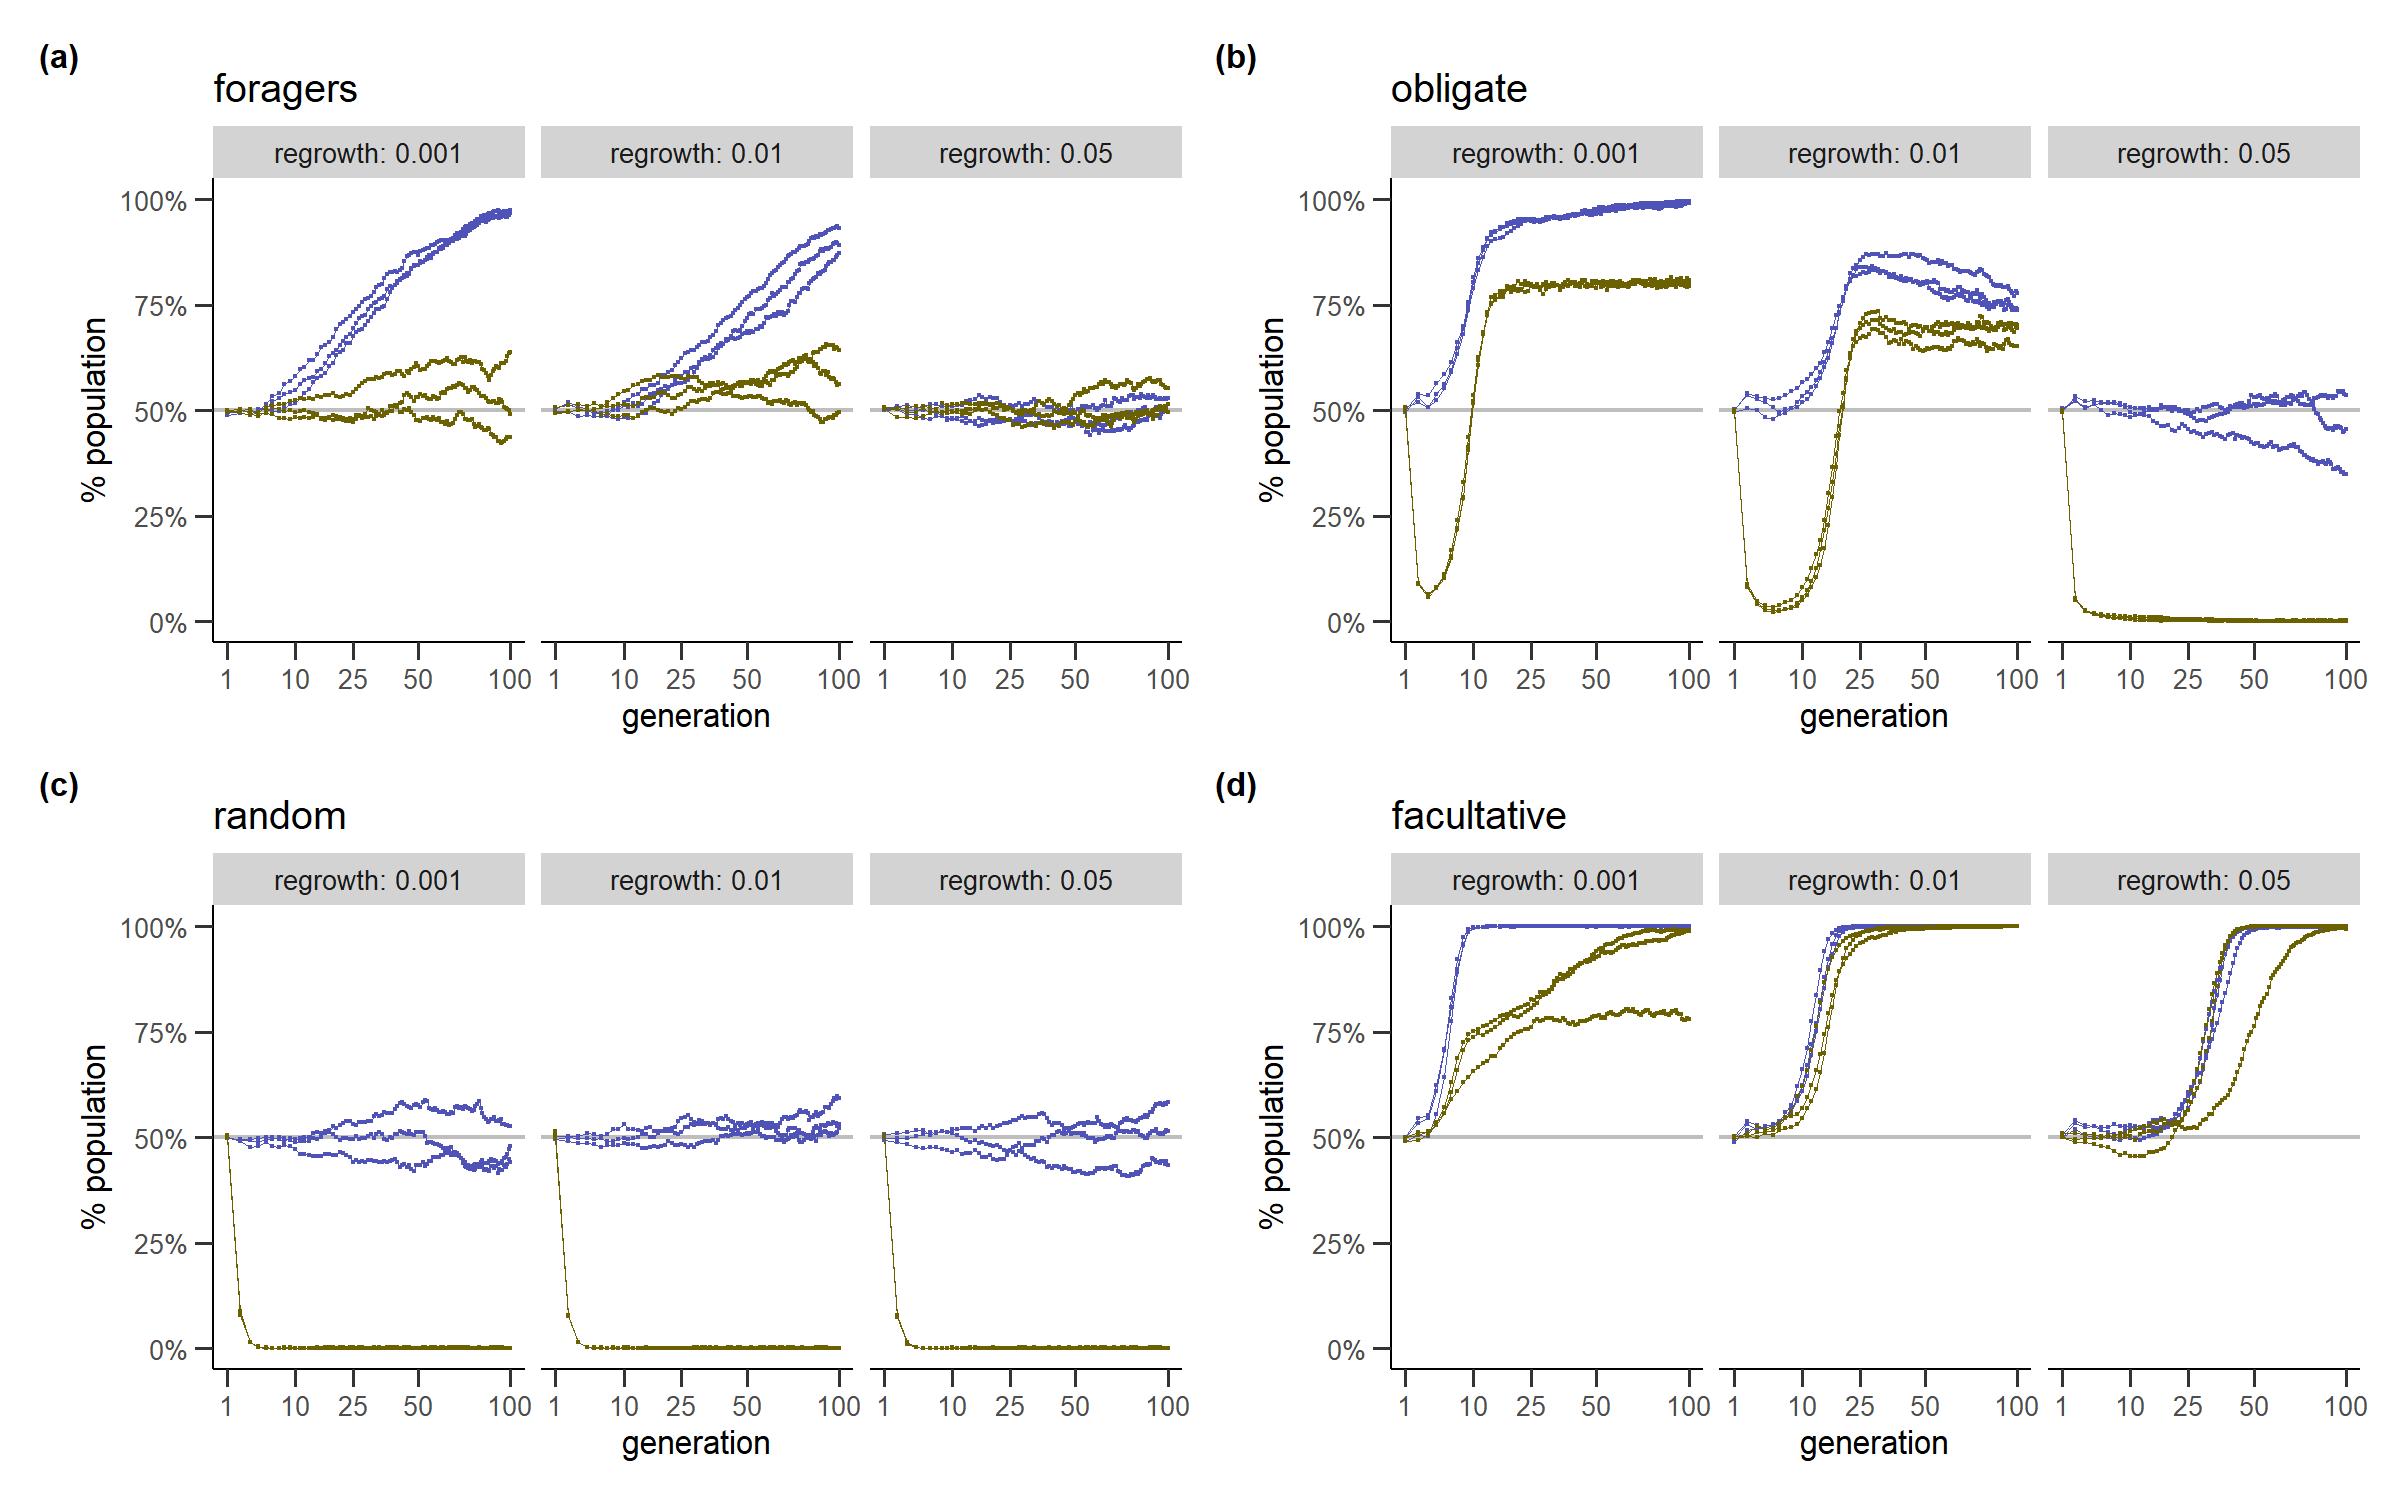
\includegraphics[width=0.90\textwidth]{figures/fig_03_preadaptation.png}
    \caption{Directed movement towards handlers is a prerequisite for the evolution of kleptoparasitism as a fixed strategy.
    \textbf{(a)} Handler preference (blue) is related to regrowth rate in scenario 1; moving towards handlers becomes universal at intermediate $r_{max}$, but decreases to 50\% at high $r_{max}$.
    The strategy bias (yellow) evolves neutrally when individuals can only forage.
    \textbf{(b)} Handler preference decreases, and takes longer to evolve with increasing $r_{max}$ in scenario 2.
    The prevalence of fixed-kleptoparasitism (yellow; strategy bias) lags the handler preference, and is very low when movement towards handlers does not evolve.
    \textbf{(c)} When individuals with fixed-strategies are forced to move randomly, handler preference evolves neutrally, and individuals inheriting a kleptoparasitic strategy go extinct.
    \textbf{(d)} In scenario 3, foraging strategy is conditioned on local conditions; individuals evolve a strong handler preference. 
    The evolved preference for stealing in the presence of handlers (yellow) does not lag the preference for moving towards handlers (blue).
    }
    \label{Fig:HandlerPreferenceBeforeKlept}
\end{figure}

\begin{figure}[h!]
    \centering
    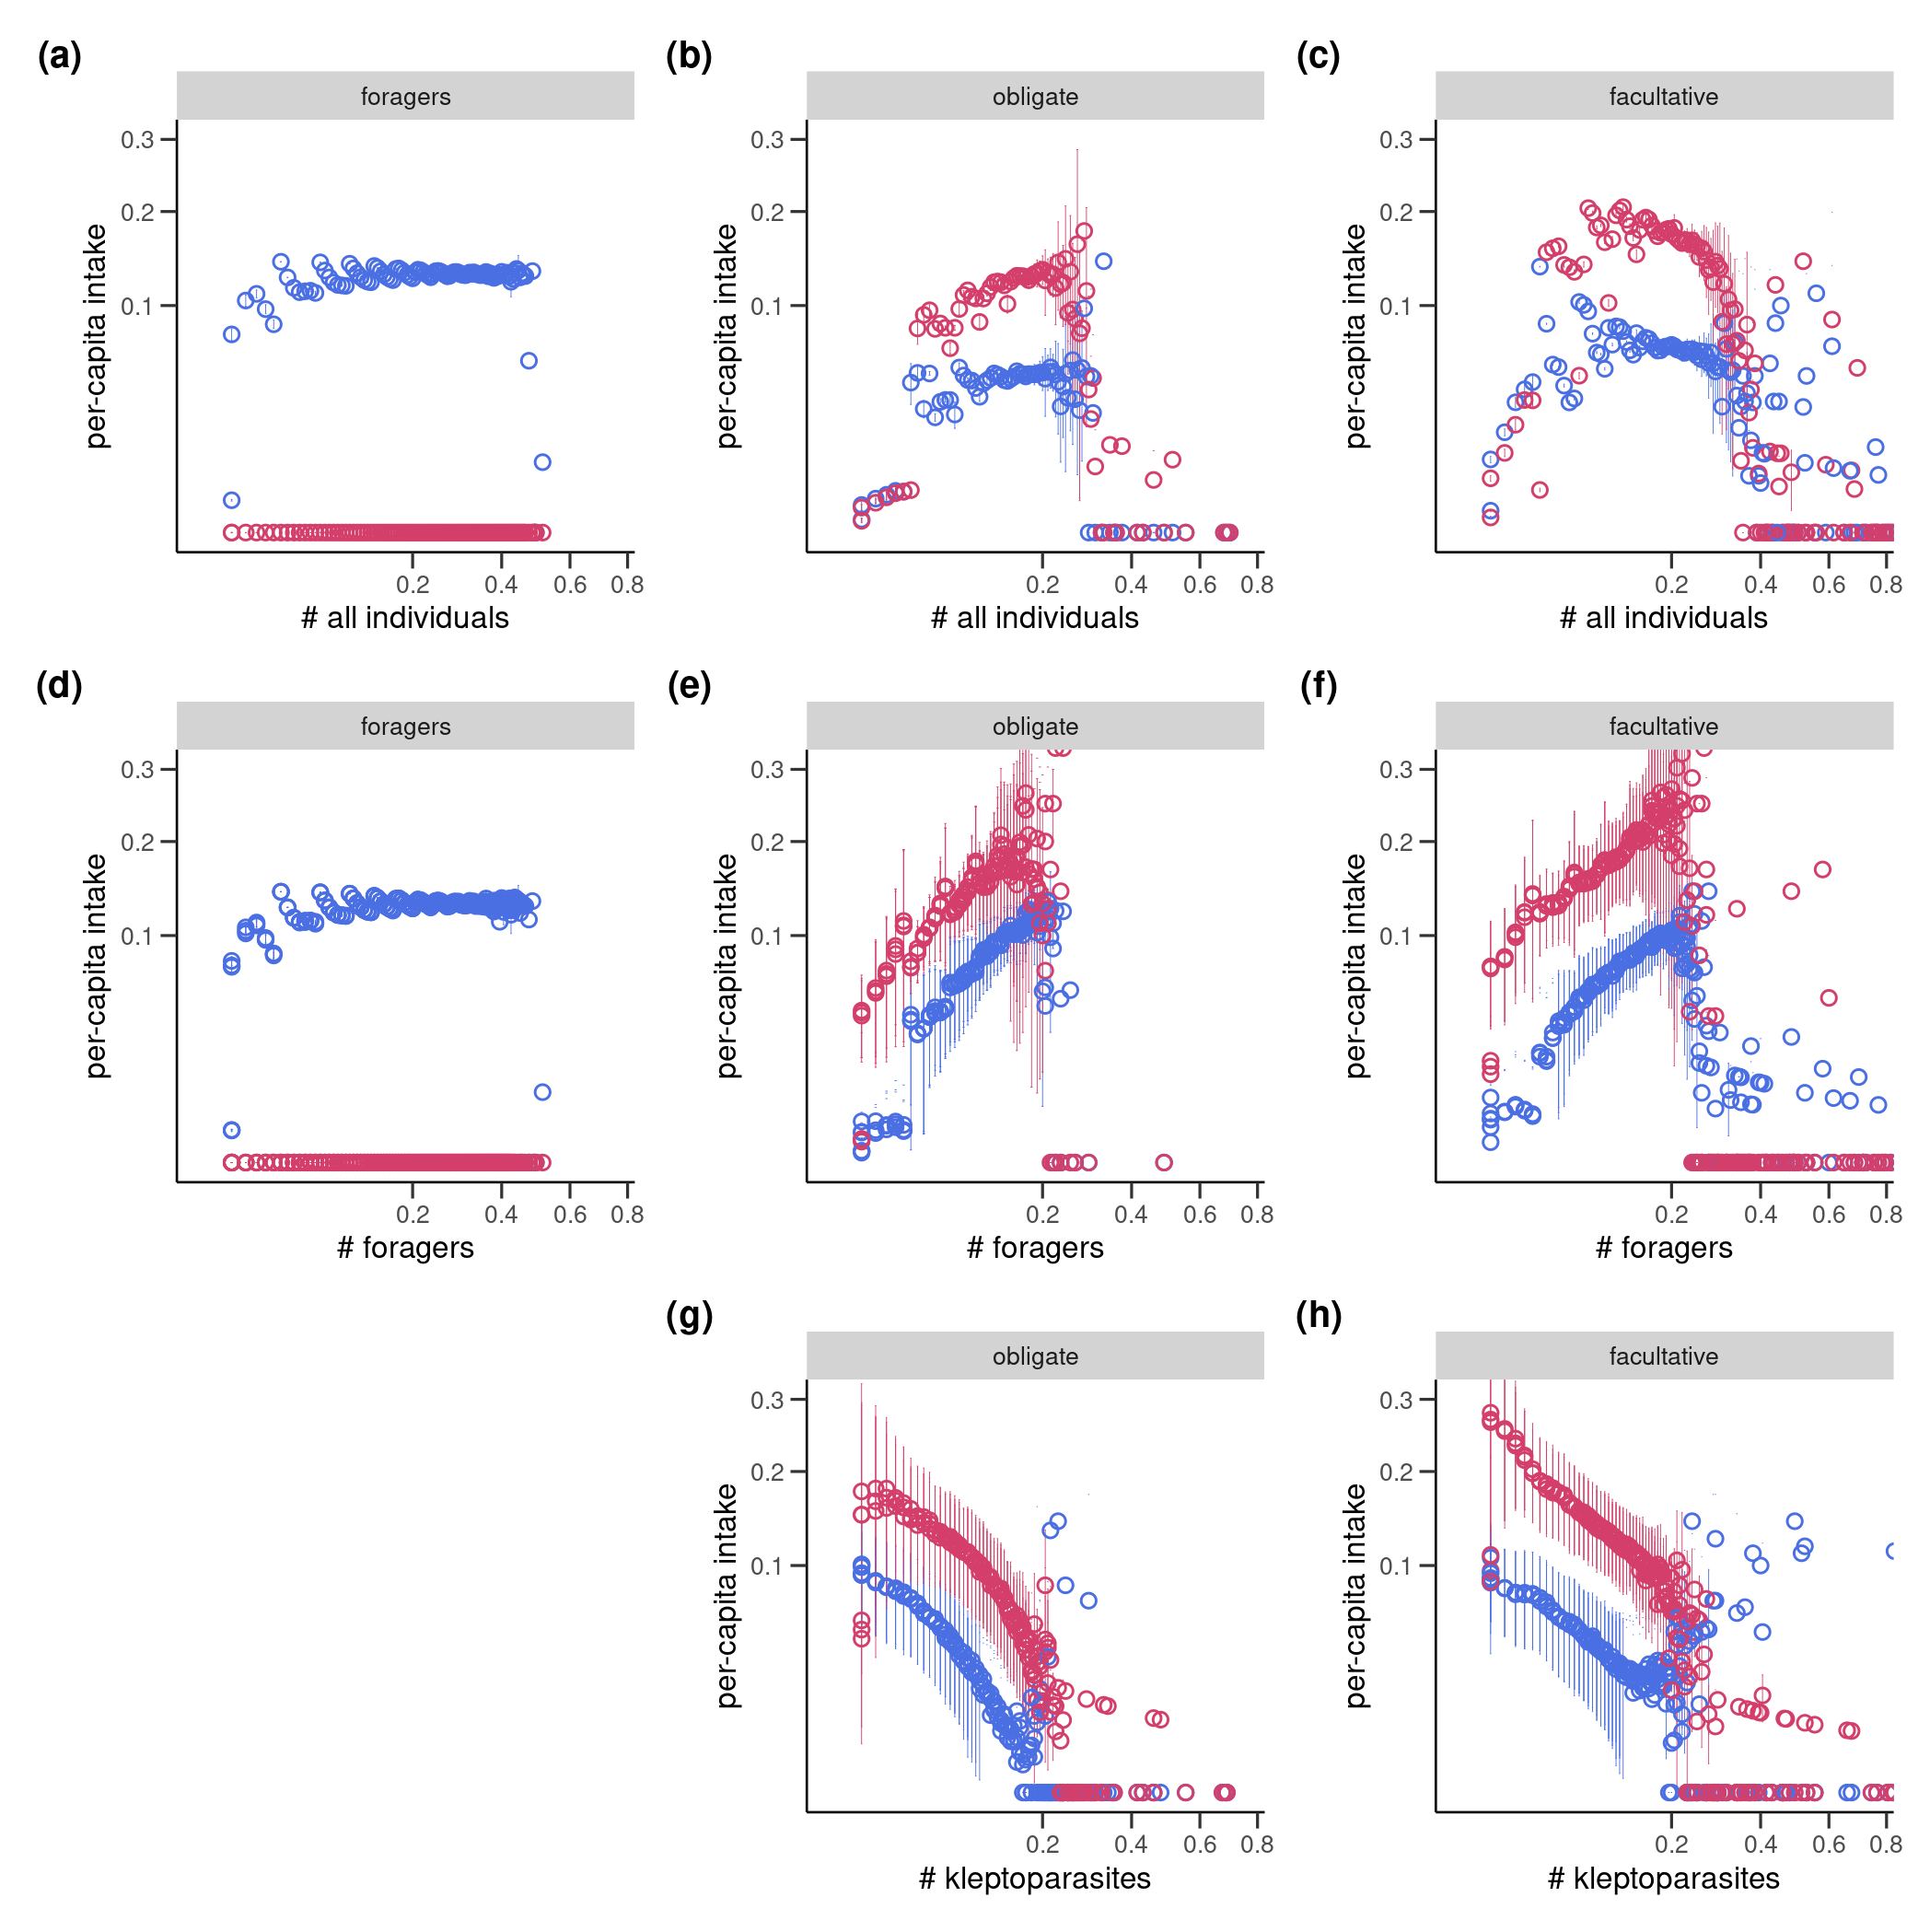
\includegraphics[width=0.90\textwidth]{figures/fig_04_functional_response.png}
    \caption{The functional response of intake to competitor density depends on competitor strategy.
    The kleptoparasite intake rate (red) is always higher than the forager intake rate (blue) on average, when Kleptoparasitism is allowed.
    \textbf{(a, b, c)} The intake rate of both strategies is approximately quadratic in relation to the density of all individuals.
    However, this quadratic response consists of \textbf{(d, e, f)} a mostly positive response of intake to increasing forager density, and \textbf{(g, h)} a strong negative response to kleptoparasite density.
    Scenarios are shown in columns (a,d = foragers-only; b, e, g = fixed-strategy; c, f, h = conditional-strategy), with $r_{max}$ = 0.1.
    }
    \label{Fig:FunctionalResponse}
\end{figure}

\begin{figure}[h!]
    \centering
    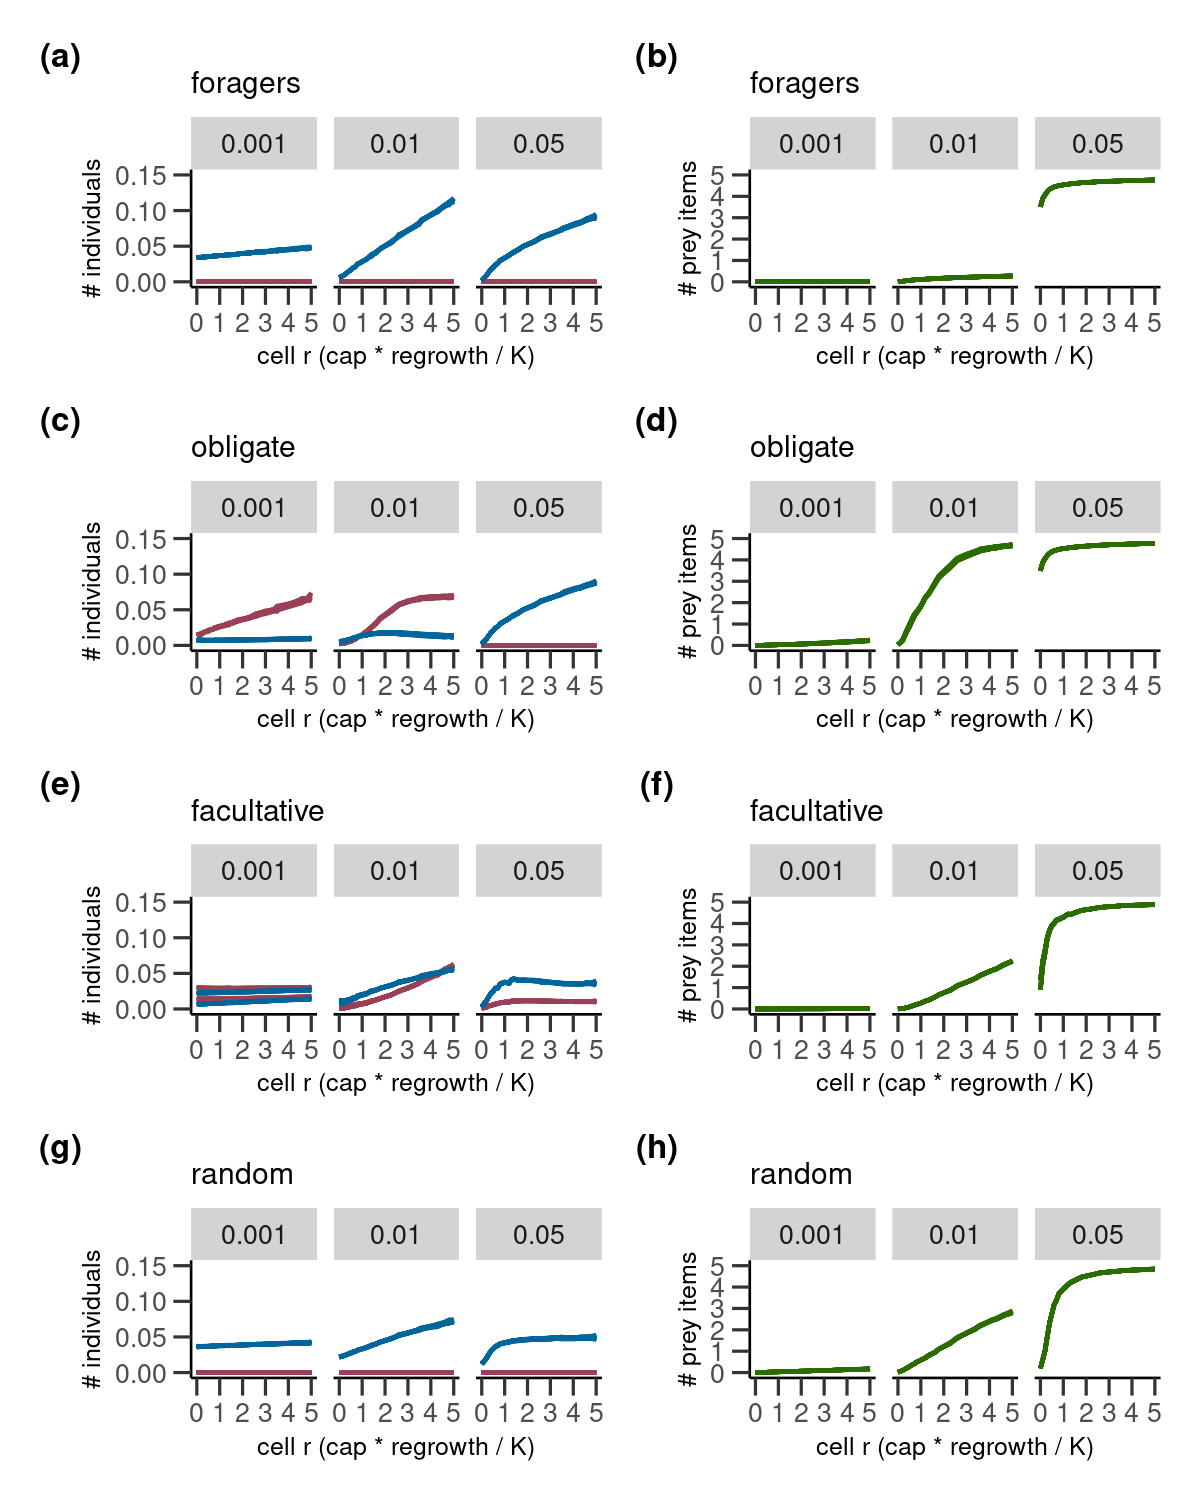
\includegraphics[width=0.90\textwidth]{figures/fig_05_agent_distribution.png}
    \caption{Population distribution in relation to landscape productivity.
    \textbf{()}}
    \label{Fig:AgentDistribution}
\end{figure}

%%%%%%%%%%%%%%%%%%%%%
% Videos
%%%%%%%%%%%%%%%%%%%%%
% If you have videos, journal style for them is similar to that for
% figures. You'll want to include a still image (such as a JPEG)
% to give your readers a preview of what the video looks like.

%%%%% Include the text below if you have videos

\renewcommand{\figurename}{Video} 
\setcounter{figure}{0}
% Thanks to Flo Debarre for the pro tip of putting
% \renewcommand{\figurename}{Video} before the Video legend and
% \renewcommand{\figurename}{Figure} after it!

% \begin{figure}[h!]
% %\includegraphics{VideoScreengrab.jpg}
% \caption{Video legends can follow the same principles as figure legends. Counters should be set and reset so that videos and figures are enumerated separately.}
% \label{VideoExample}
% \end{figure}

\renewcommand{\figurename}{Figure}
\setcounter{figure}{1}

%%%%% Include the above if you have videos


% \begin{figure}[h!]
% %\includegraphics{elegance}
% \caption{In this way, figure legends can be listed at the end of the document, with references that work, even though the graphic itself should be included for final files after acceptance. Instead, upload the relevant figure files separately to Editorial Manager; Editorial Manager should insert them at the end of the PDF automatically.}
% \label{Fig:AnotherFigure}
% \end{figure}

\subsection{Online figure legends}

\renewcommand{\thefigure}{A\arabic{figure}}
\setcounter{figure}{0}

% \begin{figure}[h!]
% %\includegraphics{jumps20m}
% \caption{\textit{A}, the quick red fox proceeding to jump 20~m straight into the air over not one, but several lazy dogs. \textit{B}, the quick red fox landing gracefully despite the skepticism of naysayers.}
% \label{Fig:Jumps}
% \end{figure}

% \begin{figure}[h!]
% %\includegraphics{jumps20m}
% \caption{The quicker the red fox jumps, the likelier it is to land near an okapi. For further details, see \citet{LemKapEx07}.}
% \label{Fig:JumpsOk}
% \end{figure}

\renewcommand{\thefigure}{B\arabic{figure}}
\setcounter{figure}{0}

\end{document}
